\documentclass[11pt]{article}

\usepackage[top=1in, bottom=1in, left=1in, right=1in]{geometry}
\usepackage{hanging}
\usepackage{amsfonts, amsmath, amssymb}
\usepackage[none]{hyphenat}
\usepackage{fancyhdr}
\usepackage[nottoc, notlot, notlof]{tocbibind}
\usepackage{graphicx}
\graphicspath{{./images/}}
\usepackage{float}

\pagestyle{fancy}
\fancyhead{}
\fancyfoot{}
\fancyhead[L]{SINGLE-VARIABLE INTEGRATION AND LINE INTEGRATION}
\fancyhead[R]{\thepage}
\fancypagestyle{firstpage}{\lhead{Running head: SINGLE-VARIABLE INTEGRATION AND LINE INTEGRATION}\rhead{\thepage}}
\renewcommand{\headrulewidth}{0pt}

\setlength{\parindent}{1.27cm}
\setlength{\parskip}{8pt}
\renewcommand{\baselinestretch}{2}

\newcommand{\ihat}{\boldsymbol{\hat{\textbf{\i}}}}
\newcommand{\jhat}{\boldsymbol{\hat{\textbf{\j}}}}
\newcommand{\dr}{\vec{r}~^{\prime}(t)}
\newcommand{\dx}{x^{\prime}(t)}
\newcommand{\dy}{y^{\prime}(t)}

\begin{document}

\thispagestyle{firstpage}
\setcounter{page}{1}
\null
\vspace{2.5cm}
\begin{center}

Single-variable integration and line integration over conservative vector fields: an analysis of the Fundamental Theorem of Calculus and the Fundamental Theorem for Line Integrals

How is the intuition in taking integrals of single-variable functions and line integrals over conservative vector fields related by the Fundamental Theorem of Calculus and the Fundamental Theorem for Line Integrals?

Mathematics

$3748$ Words

\end{center}
\vfill
%\pagebreak

%{\centering{}Abstract

%}
\pagebreak

{\centering{}Table of Contents

}
\begin{tabbing}
%Abstract \hspace{14.58cm} \= 2\\
Introduction \hspace{13.98cm} \= 3\\
Single-Variable Functions \> 4\\
~~~~The Fundamental Theorem of Calculus \> 5\\
Multivariable (Vector-valued) Functions \> 11\\
~~~~The Fundamental Theorem of Line Integrals \> 12\\
Conclusion \> 23\\
References \> 24\\
\end{tabbing}
\pagebreak

{\centering{}Single-variable integration and line integration over conservative vector fields: an analysis of the Fundamental Theorem of Calculus and the Fundamental Theorem for Line Integrals

}

Integration by antidifferentiation is a process with many intuitive interpretations; the most popular being a geometric one that connects the rate of change of the accumulation of area with the function one is integrating over. Upon considering multivariable functions, we find many more interpretations of integrals. Area under the curve could instead be volume, surface area, arclength, mass, and more. With vector-valued functions, we can sum dot products, which can be interpreted as the work done on a particle by a force field, for example.

There are theorems that govern integrating single-variable functions and multivariable functions via antidifferentiation, mainly the Fundamental Theorem of Calculus (FTC). For multivariable functions, the simplest one is the Fundamental Theorem for Line Integrals (FTLI). This theorem can be considered as a “higher-dimensional version" (Stewart, 2016) of the FTC, for particular vector-valued functions. It concerns itself with a unique kind of integral because it does not simply sum over a closed interval of one independent variable, but rather one that sums a dot product of two vector-valued functions.

Both of these theorems indicate that we can simplify the definite integral of a function into a difference of the antiderivatives of the function evaluated at the endpoints of the domain. Both processes involve taking an antiderivative to form an accumulation function. For single-variable functions the accumulation function represents signed area under the curve, whereas line integrals represent an accumulation of the sum of scalars that come from a dot product. The intuition in the FTC and the FTLI is connected because the line integrals for which the FTLI apply to are in a form that we can represent as an integral of a composite "single-variable" function for which the evaluation theorem of the FTC applies to. This idea only works as a result of fulfilling the conditions of the FTLI; however, the nature of line integrals is still different from that of single-variable integration due to some properties of vector fields. 

{\centering{}\textbf{Single-Variable Functions}

}

%In order to understand integration, we have to consider the relevant kinds of functions. Single-variable functions are different from parametric relations, which can be unlike vector-valued functions. These kinds of functions are related through the idea that functions are formal relationships between inputs and outputs.

%Functions with a single variable as its input and a single variable as its output are like "machine[s]" (Stewart, 2016) that take some input values and return corresponding output values after modifying the initial value.  A function $f$ "is a rule that assigns a unique element in $R$ to each element in $D$," (Finney, R. L., Demana, F. D., Waits, B. K., \& Kennedy, D., 2012) where $D$ is the domain or "input pool" for $f$, and $R$ is the range or "output pool" of $f$.
%how to center caption ? reduce its font?
%\begin{figure}[h]
%\center{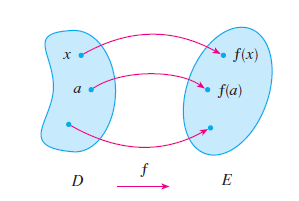
\includegraphics[scale=1]{bijection}}
%\end{figure}

%Functions are analyzed in calculus using (primarily) differentiation and integration. The derivative is analogous to slope, but can be used to find the slope of a tangent line (Finney, et al., 2012). From a different perspective the derivative can be used to measure how sensitive the function's output is (Sanderson, 2016). So for small changes in the input, we can see how much the output of the function tends to vary in response. An intuitive example of this relationship is how velocity is a time derivative of position.

The (single-variable) integral is naturally interpreted geometrically, as a result of how it is defined. The definite integral of some function is an expression that can represent the area under the graphical curve of the function bounded by the independent variable axis. It is derived from a limit of a sum of a product. Consider the Riemann sum definition of the definite integral:

$$I = \lim_{||P||\to{0}}\sum_{k=1}^n{f(c_k)\Delta{x}}$$

Quantity $I$ is the value of the definite integral, $||P||$ is the norm of the partition $P$ of the interval $[a,b]$ - the maximum distance between consecutive $c_k$ in $[a,b]$. The quantity $\Delta{x}$ is defined to be that distance between each $c_k$, $(c_k-c_{k-1})$. (Finney, R. L., Demana, F. D., Waits, B. K., \& Kennedy, D., 2012) The product that is being summed can be seen as the area of a rectangle whose base is $\Delta{x}$ and whose height is $f(c_k)$. The approximation of the area under the curve formed by the sum improves with a smaller $||P||$ until it is perfect.

%approximation improvement, new figure
\begin{figure}[h]
\centering
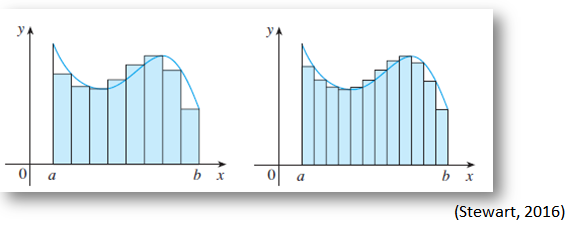
\includegraphics[scale=0.75]{approx}
\end{figure}

The image above illustrates the improvement of the approximation as the length of the largest subinterval shrinks (here the subintervals are of equal length, but that does not matter). The collection of rectangles on the right seems to better capture the area under the curve.

Taking the limit, the Riemann sum becomes the definite integral:

$$I = \int_{a}^{b}{f(x)\mathrm{d}x}$$

To show that the definite integral is evaluated through antidifferentiation, we invoke the FTC.

Theorem:
$$f(x) = \frac{\mathrm{d}}{\mathrm{d}x}\int_{a}^{x}{f(t)\mathrm{d}t}$$

Proof: Let some function represent the \textit{accumulation} of area under a curve:

$$F(x) = \int_{a}^{x}{f(t)\mathrm{d}t}$$

The continuous function $F$ represents the total area under the curve formed by the continuous function $f(t)$ bounded by the "$t$" axis from $a$ to $x$.(Johnson, 2010) We can let $f(t)$ be defined over any interval so long as it is Riemann integrable over the closed interval $[a,b]$ where $a\leq{x}\leq{b}$. Taking its derivative:

$$\frac{\mathrm{d}F}{\mathrm{d}x} = \frac{\mathrm{d}}{\mathrm{d}x}\int_{a}^{x}{f(t)\mathrm{d}t}$$
$$\frac{\mathrm{d}F}{\mathrm{d}x} = \lim_{h\to{0}}{\frac{\int_{a}^{x+h}{f(t)\mathrm{d}t}-\int_{a}^{x}{f(t)\mathrm{d}t}}{h}}$$
$$\frac{\mathrm{d}F}{\mathrm{d}x} = \lim_{h\to{0}}{\frac{\int_{a}^{x}{f(t)\mathrm{d}t}+\int_{x}^{x+h}{f(t)\mathrm{d}t}-\int_{a}^{x}{f(t)\mathrm{d}t}}{h}}$$

Then:
$$\frac{\mathrm{d}F}{\mathrm{d}x} = \lim_{h\to{0}}{\frac{\int_{x}^{x+h}{f(t)\mathrm{d}t}}{h}}$$
\begin{center}
or
\end{center}
$$\frac{\mathrm{d}F}{\mathrm{d}x} = \lim_{h\to{0}}{\frac{1}{h}\int_{x}^{x+h}{f(t)\mathrm{d}t}}$$

We use the Mean Value Theorem (MVT) for definite integrals, since $F$ is continuous. The average value of a continuous function $f$, over a closed interval $[a,b]$, is guaranteed to be some $f(c)$, for $c\in [a,b]$.(Finney, et al., 2012) Follow with the example image:

\begin{figure}[h]
\centering
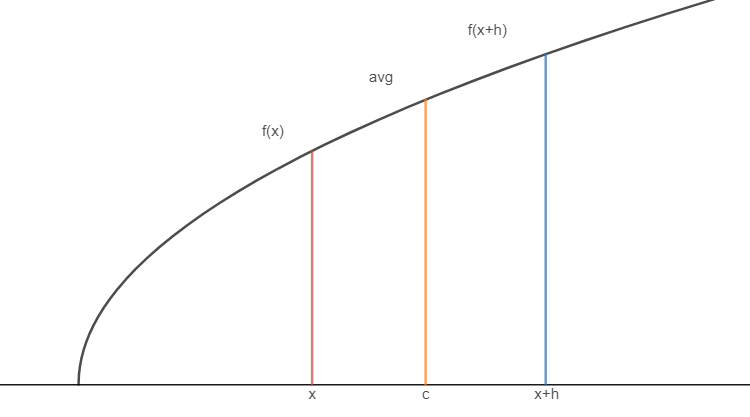
\includegraphics[scale=0.5]{squeeze}
\end{figure}

$$\lim_{h\to{0}}f(c) = \lim_{h\to{0}}{\frac{1}{h}\int_{x}^{x+h}{f(t)\mathrm{d}t}}$$
\begin{center}
or
\end{center}
$$\lim_{h\to{0}}f(c) = \lim_{h\to{0}}{\frac{1}{(x+h)-(x)}\int_{x}^{x+h}{f(t)\mathrm{d}t}}$$

By definition, and from observation in the example image, $c$ is in the interval $[x,(x+h)]$:
$$x\leq c\leq (x+h)$$

Taking the limit on the left hand side, of $f(c)$, apply the Squeeze Theorem:

$$\lim_{h\to 0}f(c)\to f(\lim_{h\to 0} c)$$
$$\lim_{h\to 0} x\leq \lim_{h\to 0} c\leq \lim_{h\to 0} (x+h)$$
$$x\leq c\leq x$$
$$c = x$$
\begin{center}
thus
\end{center}
$$\lim_{h\to 0}f(c) = f(x)$$

This use of the Squeeze Theorem is legitimate because $f$ is continuous. (Jones) Since $\displaystyle{\lim_{h\to{0}}{\frac{1}{h}\int_{x}^{x+h}{f(t)\mathrm{d}t}}}$  is simply $\displaystyle{\frac{\mathrm{d}F}{\mathrm{d}x}}$, then:

$$f(x) = \frac{\mathrm{d}F}{\mathrm{d}x}$$
\begin{center}
or
\end{center}
$$f(x) = \frac{\mathrm{d}}{\mathrm{d}x}\int_{a}^{x}{f(t)\mathrm{d}t}$$

It follows logically that the integral in this form must be an antiderivative, since it returns the function $f$ in a family of the same function (Peyam, 2019) after differentiation. Most functions are antidifferentiable if they are continuous, but there are also an infinite number of non-antidifferentiable functions.

Applying the previous result, we continue with the next part of the FTC:

Theorem:
$$\int_{a}^{b}f(t)\mathrm{d}t = F(b) - F(a)$$

Proof: Let $\displaystyle{G(x) = \int_{a}^{x}f(t)\mathrm{d}t}$ be some antiderivative of $f(x)$, however, we know that both $F(x)$ and $G(x)$ are antiderivatives of $f(x)$. Using the MVT for derivatives, we know that since $\displaystyle{\frac{\mathrm{d}G}{\mathrm{d}x}-\frac{\mathrm{d}F}{\mathrm{d}x}}=0$ for all $x$, then: (Jerison. 2010)
$$F(x)-G(x)=C$$
$$F(x)=G(x)+C$$

Working backwards:
$$F(b)-F(a) = (G(b)+C) - (G(a)+C) = G(b)-G(a)$$
$$G(b) - G(a) = \int_{a}^{b}f(t)\mathrm{d}t - \int_{a}^{a}f(t)\mathrm{d}t$$
$$G(b) - G(a) = \int_{a}^{b}f(t)\mathrm{d}t$$
Therefore:
$$\int_{a}^{b}f(t)\mathrm{d}t = F(b) - F(a)$$

%section needs pictures reeeEEEEE
A stronger proof uses Riemann sums. Let $P$ be some partition of the interval $[a,b]$ with elements ${c_k}$ for successive $k\in\mathbb{N}$ and let $G(x)$ be defined as $\displaystyle{\int_{a}^{x}f(t)\mathrm{d}t}$. Suppose the following sum captures perfectly the area under the curve $f(t)$ from $a$ to $b$: (the following is inspired by Botsko, M., and  Gosser, R.'s (1986) proof) 

(1)$$G(b)-G(a) = \sum_k{G(c_k)-G(c_{k-1})}$$ %pic, area added perfectly for arbitrary partition

Expanding the sum returns the left hand side in terms of elements of the partition $P$, for any $||P||$.\newpage

For just one section of the curve, within any $[c_{k-1},c_k]$,the following is true by application of the Extreme Value Theorem: There are values $p_k$ and $q_k$ within the interval $[c_{k-1},c_k]$ for which the average value of the area of that section is in between (or at) the heights $f(p_k)$ and $f(q_k)$. Consider one such example visually:

%picture lol
\begin{figure}[h]
\centering
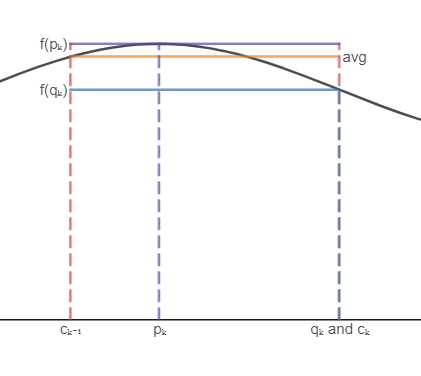
\includegraphics[scale=0.75]{darboux}
\end{figure}

The expression $\displaystyle{\frac{G(c_k)-G(c_{k-1})}{c_k-c_{k-1}}}$ is the average "height" of a section ("area" divided by length; in the example image it is the yellow height):

$$f(p_k)\leq \frac{G(c_k)-G(c_{k-1})}{c_k-c_{k-1}}\leq f(q_k)$$

Multiply by $c_k-c_{k-1}$:
$$f(p_k)(c_k-c_{k-1})\leq G(c_k)-G(c_{k-1})\leq f(q_k)(c_k-c_{k-1})$$

The left and right hand sides become the upper and lower approximations of the area under the curve section. We can sum these sectional sums over the interval and get lower and upper approximations of the integral:

$$\sum_k f(p_k)(c_k-c_{k-1})\leq \sum_k G(c_k)-G(c_{k-1})\leq \sum_k f(q_k)(c_k-c_{k-1})$$

For each sum we can let  $||P||$ tend toward $0$, which for the right and left sides involves applying the Riemann sum definition of the integral:

$$\lim_{||P||\to 0}\sum_k f(p_k)(c_k-c_{k-1}) = \int_{a}^{b}{f(t)\mathrm{d}t}$$
$$\lim_{||P||\to 0}\sum_k f(q_k)(c_k-c_{k-1}) = \int_{a}^{b}{f(t)\mathrm{d}t}$$

We take the limit and substitute identity (1):
$$\lim_{||P||\to 0}\sum_k f(p_k)(c_k-c_{k-1})\leq \lim_{||P||\to 0} \sum_k G(c_k)-G(c_{k-1})\leq \lim_{||P||\to 0}\sum_k f(q_k)(c_k-c_{k-1})$$

$$\int_{a}^{b}{f(t)\mathrm{d}t}\leq G(b)-G(a)\leq \int_{a}^{b}{f(t)\mathrm{d}t}$$

This is justified because (1) is true for any partition $P$, even as $||P||$ tends to zero. Therefore:

$$\int_{a}^{b}{f(t)\mathrm{d}t} = G(b)-G(a)$$\normalsize

The function $G$ is an antiderivative of $f$ as a result of the first part of the FTC.

%A very similar proof involves simply breaking the definite integral's evaluation up into a sum of average heights multiplied by the length (which in this proof $\displaystyle{\lim_{h\to 0}}$ is taken directly instead of the squeezing method from the earlier proof). Using the Mean Value Theorem, as $h$ tends to zero the height tends to the height of the , and finally substituting it back into the sum. The sum takes on the form of a Riemann sum, which is the definite integral. (Bond)  FLESH THIS PROOF OUT IFF ESTA POSIBLE

With these proofs we see that antidifferentiating a function returns an accumulation function of the area under its curve, because the derivative of accumulation of area for a perfect approximation is the same class of function as the integrand. Furthermore, since we have a function to represent accumulation of area, it is intuitive to see how differences in area accumulation correspond with areas of specific regions under the curve. The second proof strengthens this idea by bounding the supposed area defined by antiderivatives of the section under an upper and lower Riemann sum for the area under the curve; then letting the norm of the partition tend to zero. The result confirms the evaluation theorem. This geometric interpretation reappears similarly in the FTLI.

{\centering{}\textbf{Multivariable Functions}

}
%There are many kinds of multivariable functions, but only a few are relevant. Parametric relations are functions which relate the output of some function to its input by introducing a parameter, in which the input and output are functions of the parameter. For some function $f$ a parameterization could be:

%$$f(x)=g(t)~\text{or}~f(h(t))$$
%$$x=h(t)$$
%

%It is important to note that this process changes the single-variable function $f$ into a sort of multivariable function where $t$ is the input and the values $x$, $f(x)$ are the outputs. Another example: %picture?

%$$f(x,y)=f(h(t),g(t))$$
%$$x=h(t)$$
%$$y=g(t)$$
%

%Furthermore these relations are generally graphed with the outputs as axes (the parameter is not usually an axis). Going up a level we find we have full-fledged multivariable functions, whose inputs are values from (potentially) more than one variable, and whose outputs are values from (potentially) more than one dependent variable. We can integrate and differentiate them, however, specificity of which variable is being analyzed is required. For differentiation, partial differentiation is used to denote the idea that it's only a measure of part of the function's behavior. Integrals already have the notation required to be specific.

Vector-valued functions, like most parametric relationships, use different functions of one or more variables/parameters, but form vectors whose direction and magnitude change with those variables/parameters. It forms vectors that can begin either at the origin or at points in the output space, pointing to someplace else as a result of its direction and magnitude. Vector-valued functions are called vector fields when they produce vectors at every point in an $\mathbb{R}^n$ output space. (Dawkins, 2018)

%There are proprietary operations for vectors like the dot and cross products that return scalar and vector quantities, respectively. The dot product of two vectors $\vec{a}$ and $\vec{b}$ is the sum of the products of their corresponding components:
%$$\vec{a}= a_x\ihat+a_y\jhat$$
%$$\vec{b}= b_x\ihat+b_y\jhat$$
%$$\vec{a}\cdot\vec{b} = a_xb_x + a_yb_y$$

The process of integrating using vector-valued functions looks quite different from simply integrating scalar valued functions, but the intuition is closely related.

Line integration is a form of integration in multidimensional space, in which integration with respect to not one axis, but multiple axes, is permitted - specifically integrating with respect to changes in a particular path in multiple axes at once. Consider $f(x,y)$, integrated not over an interval in the $x$ axis nor the $y$ axis, but over a curve $C$. This path can be defined by a parametric relation, $r(t)$ for some interval of $t$. Going back to single-variable notions, we would want to sum the product of the function evaluated at every point on that curve with a small change in the curve, which here can be expressed as an arclength element. An example line integral might look like the following, with the orange curve defined with $r(t)$:

\begin{figure}[h]
\centering
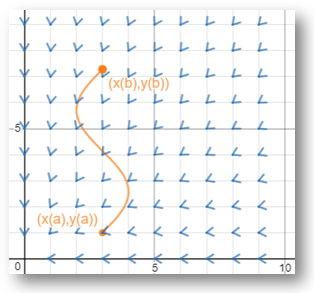
\includegraphics[scale=0.75]{lineint}
\end{figure}

For the Fundamental Theorem of Line Integrals, there are no scalar functions immediately present: there is a vector field and the path integrated over is defined by a vector-valued function (and/or a parametric relation) over a time interval. The proof of the FTLI shows how we can still integrate with a similar intuition to scalar integration. (Dawkins, 2018; Stewart, 2016)

Theorem:
$$\int_C \vec{F}\cdot\mathrm{d}\vec{r}(t) = f(\vec{r}(b))-f(\vec{r}(a))$$

Vector field $\vec{F}$ is conservative, and $C$ denotes that we are integrating over its path traced by $\vec{r}(t) = x(t)\ihat+y(t)\jhat$ for $t\in [a,b]$, having endpoints at $\vec{r}(a)$ and $\vec{r}(b)$. It should be noted that we shouldn't really evaluate $f$ at the terminal points of vectors; in which case the less compact notation involves writing the right hand side as $f(x(b),y(b))-f(x(a),y(a))$ where $x(t)$ and $y(t)$ are the components of $\vec{r}(t)$ that trace out the $x$ and $y$ coordinates of the curve $C$. This is a result of simultaneously defining the curve $C$ with both a vector-valued function and a parametric relation.\newpage

%pic lol

To be conservative, a vector field must be formed with the gradient operator. The gradient of a scalar function $f(x,y)$ is:

$$\nabla f(x,y) = \frac{\partial f}{\partial x}\ihat + \frac{\partial f}{\partial y}\jhat$$

An example of the gradient is of a paraboloid:

\begin{figure}[h]
\centering
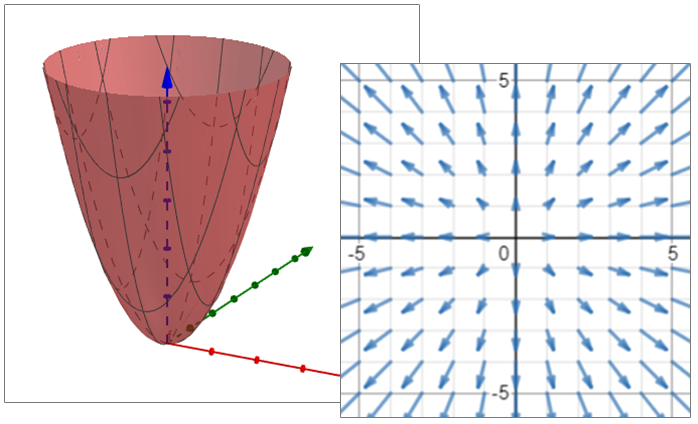
\includegraphics[scale=0.75]{gradient}
\end{figure}

Briefly consider how the single-variable derivative is analogous to slope, but can be used to find the slope of a tangent line (Finney, et al., 2012). From a different perspective the derivative can be used to measure how sensitive the function's output is (Sanderson, 2016). So for small changes in the input, we can see how much the output of the function tends to vary in response. When this derivative is positive it means the function is increasing, and when it is negative the function is decreasing (meaning a unit step backward in the independent variable would produce an increase in the function). The same thing happens with the gradient - the vectors in the vector field formed by the gradient will point in the direction which produces the "steepest ascent" (Sanderson, 2016) of $f$. This is because when the partial derivative is positive, it implies that a positive change in the axis it differentiates with respect to will increase the value of $f$, and vice versa with a negative partial derivative. The magnitude of any particular vector found in the vector field formed by $\nabla f(x,y)$ indicates the actual sensitivity of the function, which increases with an increased change in the dependent variable for a given step in its direction, much like in the single variable case. Hence the gradient is analogous to the derivative. We continue with the proof.

Thus we can rewrite the integral $\displaystyle{\int_C \vec{F}\cdot\mathrm{d}\vec{r}(t)}$ into:

$$\int_C \nabla f(x,y)\cdot \mathrm{d}\vec{r}(t)$$

We want to have the function evaluated on the points on the curve $C$, like we do with standard integration - except over the interval on the axis. We proceed by "forcing" the input of the vector field to be $x(t),y(t)$ rather than all $x,y$. This is a result of defining the curve $C$ as a parametric relation of $x$ and $y$ based on the components of $\vec{r}(t)$.

$$\vec{r}(t)=x(t)\ihat+y(t)\jhat$$
$$y=y(t)$$
$$x=x(t)$$


Then:
$$\int_C \nabla f(x(t),y(t))\cdot \mathrm{d}\vec{r}(t)$$

Because $\displaystyle{\frac{\mathrm{d}\vec{r}(t)}{\mathrm{d}t}=\dr}$, we can use the following substitution:
$$\mathrm{d}\vec{r}(t)=\dr\mathrm{d}t$$

There is a neat intuitive explanation of why this substitution is effective. Notice how it is an application of local linearity, in which a small element of the arclength of $C$ is formed out of the above product, $\mathrm{d}t$ being a very small element of $t$. If we took an infinite sum on both sides, then we would simply get $C$ again.

We also have to note that once we do this substitution we are no longer integrating over $\vec{r}(t)$, but rather $t$ in the interval $[a,b]$, and so the bounds change:

$$\int_a^b \nabla f(x(t),y(t))\cdot \dr\mathrm{d}t$$

An example change of variables might look like the next two pictures, changing the integral from a multi-variable one to a single-variable one, where the area under the curve on the right visual would represent the value of the line integral.

\begin{figure}[h]
\centering
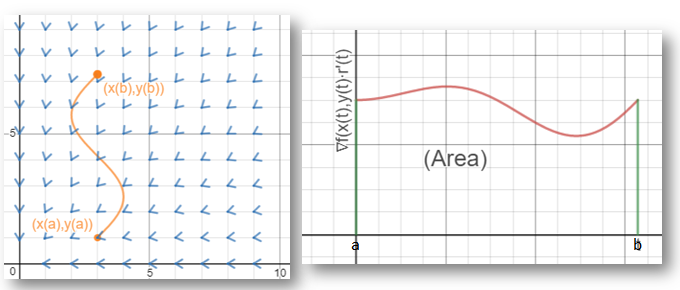
\includegraphics[scale=0.75]{cvars}
\end{figure}

Substitute in the vectors and take the dot product. Since we are essentially summing dot products in the line integral, one particular one of those dot products would be taken of these two vectors, as an example:

\begin{figure}[h]
\centering
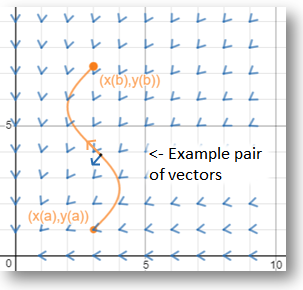
\includegraphics[scale=0.75]{dotprod}
\end{figure}

 Note that $\dr=\dx\ihat+\dy\jhat$ and the components of $\nabla f(x(t),y(t))$ are its partial derivatives.

$$\int_a^b \left[ \left(\frac{\partial f}{\partial x(t)}\ihat+\frac{\partial f(t)}{\partial y(t)}\jhat\right)\cdot (\dx\ihat+\dy\jhat)\right]\mathrm{d}t$$
$$\int_a^b\left[\frac{\partial f}{\partial x(t)}\frac{\mathrm{d}x(t)}{\mathrm{d}t}+\frac{\partial f}{\partial y}\frac{\mathrm{d}y(t)}{\mathrm{d}t}\right]\mathrm{d}t$$

Use the Multivariable Chain Rule to simplify the integrand:
$$\int_a^b \left[\frac{\mathrm{d}f}{\mathrm{d}t}\right]\mathrm{d}t$$

Apply the FTC to simplify this into:
$$f(b)-f(a)$$
\begin{center}
or more clearly
\end{center}
$$f(x(b),y(b))-f(x(a),y(a))$$

The result of the FTLI is so similar to the result of the FTC, mainly because the use of the FTC lends itself to changing the integral into the form we are familiar with. However, we can peel back layers to find that there are connections beyond just the use of the FTC, although there are other differences between the developments of the two theorems.

There are immediate similarities between line integration and single-variable integration. Consider the familiar properties of single-variable integrals:

$$\int_a^a f(x)\mathrm{d}x$$
\begin{center}
or
\end{center}
$$\int_a^b f(x)\mathrm{d}x + \int_b^a f(x)\mathrm{d}x = 0$$

A similar property is found in line integration satisfying the FTLI:

$$\oint_C \vec{F}\cdot \mathrm{d}\vec{r}(t)=0$$
\begin{center}
or
\end{center}
$$\int_a^b \nabla f(x(t),y(t))\cdot \dr\mathrm{d}t = 0$$

\newpage
Which might look like so:

\begin{figure}[h]
\centering
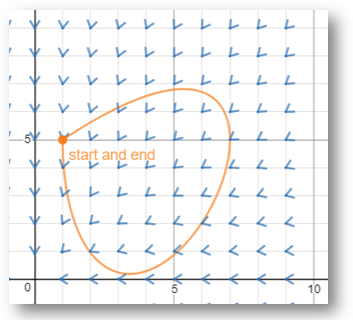
\includegraphics[scale=0.75]{loop}
\end{figure}

The curve $C$ here is closed (and simple) - the endpoints of $C$ are the same point - so the integral equals 0. This relates back to the single-variable integral sum whose path on the $x$ axis we are summing over is closed in the same way the line integral is - we go from $a$ to $b$ and back to $a$. In both example integrals the accumulation of the product reaches a value and returns to $0$.

%examples and pictures with numbers lol to make sure

Line integration over conservative vector fields and standard integration are both path independent, in that no matter how we traverse between the endpoints of the path, any extraneous motion in the path will cancel itself out, equivalent to the accumulation of the product in a direct path between the endpoints.

In the same manner another property is common. We can subdivide the paths arbitrarily, in which we sum the accumulations over the sections of the path that form the full path. For example, consider the integral $\displaystyle{\int_a^b f(x)\mathrm{d}x}$. It can be broken up into the sum of the following integrals where $c,d\in [a,b]$ and $c\leq d$.

$$\int_a^b f(x)\mathrm{d}x = \int_a^c f(x)\mathrm{d}x +\int_c^a f(x)\mathrm{d}x +\int_a^d f(x)\mathrm{d}x +\int_d^b f(x)\mathrm{d}x$$

Likewise, for $\displaystyle{C=\bigcup_{k=1}^4 C_k}$
$$\int_C \vec{E}\cdot\mathrm{d}\vec{r}(t)=\int_{C_1}\vec{E}\cdot\mathrm{d}\vec{r}(t)+\int_{C_2}\vec{E}\cdot\mathrm{d}\vec{r}(t)+\int_{C_3}\vec{E}\cdot\mathrm{d}\vec{r}(t)+\int_{C_4}\vec{E}\cdot\mathrm{d}\vec{r}(t)$$

This property of line integrals and single-variable integrals is very useful in situations where directly integrating over an interval is impossible because there is some issue with the function being integrated at one or many points in such an interval. For single-variable integrals, an obvious example is when a function is not defined at some $x$, in which case the integral would be split up into a sum of improper integrals. For line integrals, this problem can exist in and of the path itself; if the path is not simple, or it is not at least piecewise smooth somewhere - the path can be split up to resolve the issue.

Another way these theorems are related is in their requirements. To use the FTC to evaluate a single-variable integral, the antiderivative must exist. Likewise, the requirement that the vector field in the integrand of line integrals be conservative also draws on the same idea. For a vector field to be conservative, it must be the gradient of some scalar function (Riman, 2018) - the gradient being a form of a derivative, using vectors. The gradient only forms half of the kind of a derivative we are used to seeing in the integrands of single-variable integrals, in which the integrand is not some partial derivative but the entire derivative of a function, furthermore the derivative being a scalar function as well. The FTLI "completes" the derivative through the dot product. The components of the vector field $\vec{F}$ are only part of the derivative of the scalar function needed, and the components of $\dr$ are the other part - they form a total derivative of the scalar function with respect to $t$, measuring its full rate of change, only over the path of the curve.

The main point of interest is how the substitution $\mathrm{d}\vec{r}(t)=\dr\mathrm{d}t$ functions. Before this step in the proof, the line integral had still been summing over small changes in the path $C$, and with the substitution we have effectively changed a two dimensional sum into a one dimensional sum. This is further reinforced when the dot product is taken, causing both vectors to become one scalar function. The integral becomes, even though there are composite functions, a single-variable integral in which the FTC applies. We can then interpret it as a sum of rectangles, like it is with single-variable integration - except that the height is $\vec{F}\cdot\dr$ and the base is $\mathrm{d}t$.

With the FTC there was no need for simultaneously defining the interval on the $x$ axis as a vector-valued function and as a parametric relation - because the path in the $x$ axis is straightforward and is linear. Paths in the $xy$ plane can have all sorts of properties, and this becomes apparent if we consider kinematics. For example, a particle's motion in a force field has instantaneous velocities which are the tangent vectors to its path - however, another particle can take the same path and have different instantaneous velocities. If we computed the work done by the force field, we would get different results.

%There are ways to produce the same effect in a single-variable environment by letting the upper bound of some definite integral be a function of time, in which we apply the FTC with the Chain Rule to evaluate the definite integral. This kind of accumulation is not inherently a part of their integrands like it is in line integration. Recalling from the FTLI, the substitution itself changes the way the accumulation is taken.

Substitution in a single-variable integration is not uncommon, and functions the same way as it does in line integration by changing the accumulation (but not the evaluation itself). Substitutions change the input space the integral is summing over, in line integration from the path in the $xy$ plane to $t$, in single-variable integration from one axis to another axis (because a function in one axis models change in the other) - substitution transcends both of these types of integration. Using the determinant of the Jacobian matrix to convert areas of domains is not fundamentally different than scaling the lengths of intervals in single-variable integration, still no different than converting integrating over a path to over a parameter. Vector-valued functions model change in the path in the $xy$ plane the same way scalar functions might model paths in an arbitrary axis, through the derivative (and linearity).

$$\int_a^b f((u(x))u^{\prime}(x)\mathrm{d}x = \int_{u(a)}^{u(b)} f(u)\mathrm{d}u$$
\begin{center}
is like the reverse of
\end{center}$$\int_C \nabla f(x(t),y(t))\cdot \mathrm{d}\vec{r}(t) = \int_a^b \nabla f(x(t),y(t))\cdot \dr\mathrm{d}t$$

For this reason the use of the Multivariable Chain Rule forms a superficial difference in these two kinds of integration . The substitution changes the input space, filling in the rest of the "derivative" needed to form a scalar function - the use of the dot product is the more important difference between them. The original integral sums a dot product, which involves a measure of how linearly dependent the vectors are - an alternative interpretation than areas of rectangles.

There are other significant differences between the intuitions of line integration over conservative vector fields and single-variable integration. The conservative vector field required for the FTLI serves as part of a "derivative-like function" (Guichard), but the difference between this "derivative" and the integrands of single-variable integrals is that there is a test to check if some vector field is conservative or not. In single-variable integration, this would be similar to being able to check for sure if the integrand is the derivative of some other function, which allows the use of the FTC - this is not so straightforward, as there are many functions that do not have elementary antiderivatives. Proving that some function does not have an elementary antiderivative requires analysis.

The test involves taking partial derivatives of the components of the vector field, and comparing them. For two dimensional vectors we take the partial derivative of the $y$ component ($\jhat$) with respect to $x$ and vice versa with the other, and if they are equal to each other, then the field is conservative.

$$\frac{\partial \frac{\partial f}{\partial x}}{\partial y}=\frac{\partial \frac{\partial f}{\partial y}}{\partial x}~\text{or}~\frac{\partial^2f}{\partial x\partial y}=\frac{\partial^2f}{\partial y\partial x}$$

This test only works for vector fields occupying two spatial dimensions, though. The actual test involves checking if the curl of the vector field is $0$, in which case only then it is conservative, but the use of the curl operation to test the vector field is only applicable in odd numbered dimensions. %do you have a source for this ???
The simple reason for the two dimensional test being unique is that the curl operation involves the cross product, which is not defined for 2-dimensional spaces, which is why we directly take partial derivatives. If (and since) those partial derivatives are equal to each other, they are the mixed higher order partial derivatives of some scalar function. It is a reverse application of Clairaut's theorem (Lambers, 2010), which states that for continuous scalar functions (in this case $\mathbb{R}^3$), their mixed second partial derivatives must be equal to each other so long as they exist and are continuous.

This implies that a continuous scalar function exists, and therefore, the vector field is a gradient of that vector field. Mixed partial derivatives and the curl operator have no analogue in single-variable calculus, which is an indicator of how line integration is not a perfect analogue of single-variable integration. This sort of test also does not guarantee that the part of the integral evaluated with the FTC will work out, simply that the prerequisite of having a conservative vector field is confirmed. Furthermore, there are other ways to prove a vector field is conservative over a region formed by a closed and simple path, using Green's or Stokes' theorem, which are both even grander analogues of the FTC in a multivariable environment. Those applications are outside the scope of this paper.

%Green's' theorem relates a closed line integral over a vector field (which is not required to be conservative) in two dimensions to an area integral over the region the path of the integral encloses. The integrand of the area integral is the special "two dimensional curl" of the vector field.

%From the definition itself we can see how if the vector field were to be conservative, the curl of such a vector field would be zero and thus the region it encloses would have an area of zero. The more important fact is that the equivalence using Green's theorem is a different way entirely to achieve the same set of partial derivatives, that have the same implication through Clairaut's theorem that such a scalar function exists and the gradient of that function is the vector field, on all points in the region the line integral encloses. Using Green's theorem is better for guaranteeing the conservative nature of a vector field because it will check for all points, including the ones on the path - in practice it takes extra work to prove that a vector field is conservative over a full region using the curl test, because it does not consider the parts of the vector field that are not on the path indicated. See Appendix B for more information on how using Green's theorem can check if a field is conservative. For line integrals in three dimensional space outlining surfaces instead of plane regions, we use Stokes' theorem to carry out the same process. %what the actual fuck fix this please
 
\pagebreak

{\centering{}Conclusion

}
To recapitulate, the FTC relates differentiation and integration through the antiderivative, as near inverses. It works by showing that integrals as accumulation functions have a derivative of the same function as its integrand. This implies that the integral must be an antiderivative. Using the MVT or Riemann sums, we can show that the difference between accumulation functions at two points gives the area of the area under the curve between those two points. The FTLI shows that the integral of a dot product of a conservative vector field and the tangent vectors to a path $C$ in multidimensional space is equivalent to the difference of the function whose gradient is the vector field having been evaluated at the end times for which $C$ was parameterized by.
The similarities between the two kinds of integration manifest themselves in path independence, path sectionability, and antidifferentiation (through the FTC). The main difference between the kinds of integration is found in line integration, in which the quality of a vector field to be conservative, as a form of a "derivative", can be tested, which has no simple analogue for single-variable integrands. The FTLI is an expansion of the FTC.
\pagebreak

{\centering{}References

}
\begin{hangparas}{0.5in}{1}
%Bond, R. (1981). 65.42 An Alternative Proof of the Fundamental Theorem of Calculus. The Mathematical Gazette, 65(434), 288-289. doi:10.2307/3616605

Botsko, M, \& Gosser, R. (1986). Stronger Versions of the Fundamental Theorem of Calculus. \textit{The American Mathematical Monthly, 93}(4), 294-296. doi:10.2307/2323686

Dawkins, P. (2018, June 1). Section 5-1 : Vector Fields. Retrieved from http://tutorial.math.lamar\\.edu/Classes/CalcIII/VectorFields.aspx

Dawkins, P. (2018, June 1). Section 5-5 : Fundamental Theorem For Line Integrals. Retrieved from http://tutorial.math.lamar.edu/Classes/CalcIII/FundThmLineIntegrals.aspx

Finney, R. L., Demana, F. D., Waits, B. K., \& Kennedy, D. (2012). \textit{Calculus: Graphical, numerical, algebraic}(4th ed.). Boston, MA: Prentice Hall.

Riman, M. (2018, October). \textit{16.3: The Fundamental Theorem for Line Integrals over Vector Fields}[PDF]. Seattle: University of Washington.

Guichard, D. (n.d.). 16.3 The Fundamental Theorem of Line Integrals. Retrieved from https://\\www.whitman.edu/mathematics/calculus\_ online/section16.03.html

David Jerison. \textit{.01SC Single Variable Calculus.} Fall 2010. Massachusetts Institute of Technology: MIT OpenCourseWare, https://ocw.mit.edu. License: Creative Commons BY-NC-SA.

Johnson, H. (2010). Investigating the Fundamental Theorem of CALCULUS. \textit{The Mathematics Teacher,} 103(6), 430-435. Retrieved from http://www.jstor.org/stable/20876657

Jones, D. A. (n.d.). \textit{Ch4}[PDF]. Tempe: Arizona State University. Retrieved from https:/\\/math.la.asu.edu/~dajones/class/371/ch4.pdf

Lambers, J. (2010). \textit{The Fundamental Theorem for Line Integrals}[PDF]. Hattiesburg: The University of Southern Mississippi.

Sanderson, G. (2015). What are multivariable functions? Retrieved February 13, 2019, from https://www.khanacademy.org/math/multivariable-calculus/thinking-about-multivariable-function/
ways-to-represent-multivariable-functions/a/multivariable-functions

Stewart, J. (2016). \textit{Calculus} (8th ed.). Boston, MA: Cengage Learning.

Tabrizian, P. R. (2019, January 23). Retrieved February 14, 2019, from https://www.youtube.com/
watch?v=H2ytsTrKmvI
\end{hangparas}
\end{document}
